\chapter{Elementi caratterizzanti del progetto}
\label{cap:elementi-progetto}
% Qui introdurrò brevemente il contenuto delle sezioni sottostanti.
Questo capitolo si occupa di introdurre gli strumenti utilizzati nel corso del tirocinio, definire e dare una visione concreta delle attività di sviluppo del progetto di \textit{stage} e dare prova dei risultati raggiunti 
a livello di documentazione, di codice scritto, \textit{test coverage} e obiettivi raggiunti. 

\section{Stile lavorativo}

% In questa sezione descriverò il modo in cui ho lavorato nel corso del tirocinio, descrivendo attività esterne allo sviluppo, alla verifica ed alla validazione e descrivendo il modo in cui invece tali attività sono state ideate.
Data la pianificazione a cadenza settimanale delle attività (sezione \hyperref[sec:pianificazione]{§2.5}), ho concordato con il tutor aziendale, il signor \textit{Michele Rigo}, l'organizzazione di una riunione di allineamento settimanale, programmata per ogni lunedì mattina. \\
Tale incontro mirava a:
\begin{itemize}
    \item Mostrare il lavoro svolto nel corso della settimana precedente alla riunione;
    \item Condurre una retrospettiva sulla settimana precedente;
    \item Valutare lo stato di avanzamento del progetto in relazione alle aspettative;
    \item Delineare le attività da svolgere nella settimana in corso.
\end{itemize}

\begin{figure}[H]
    \centering
    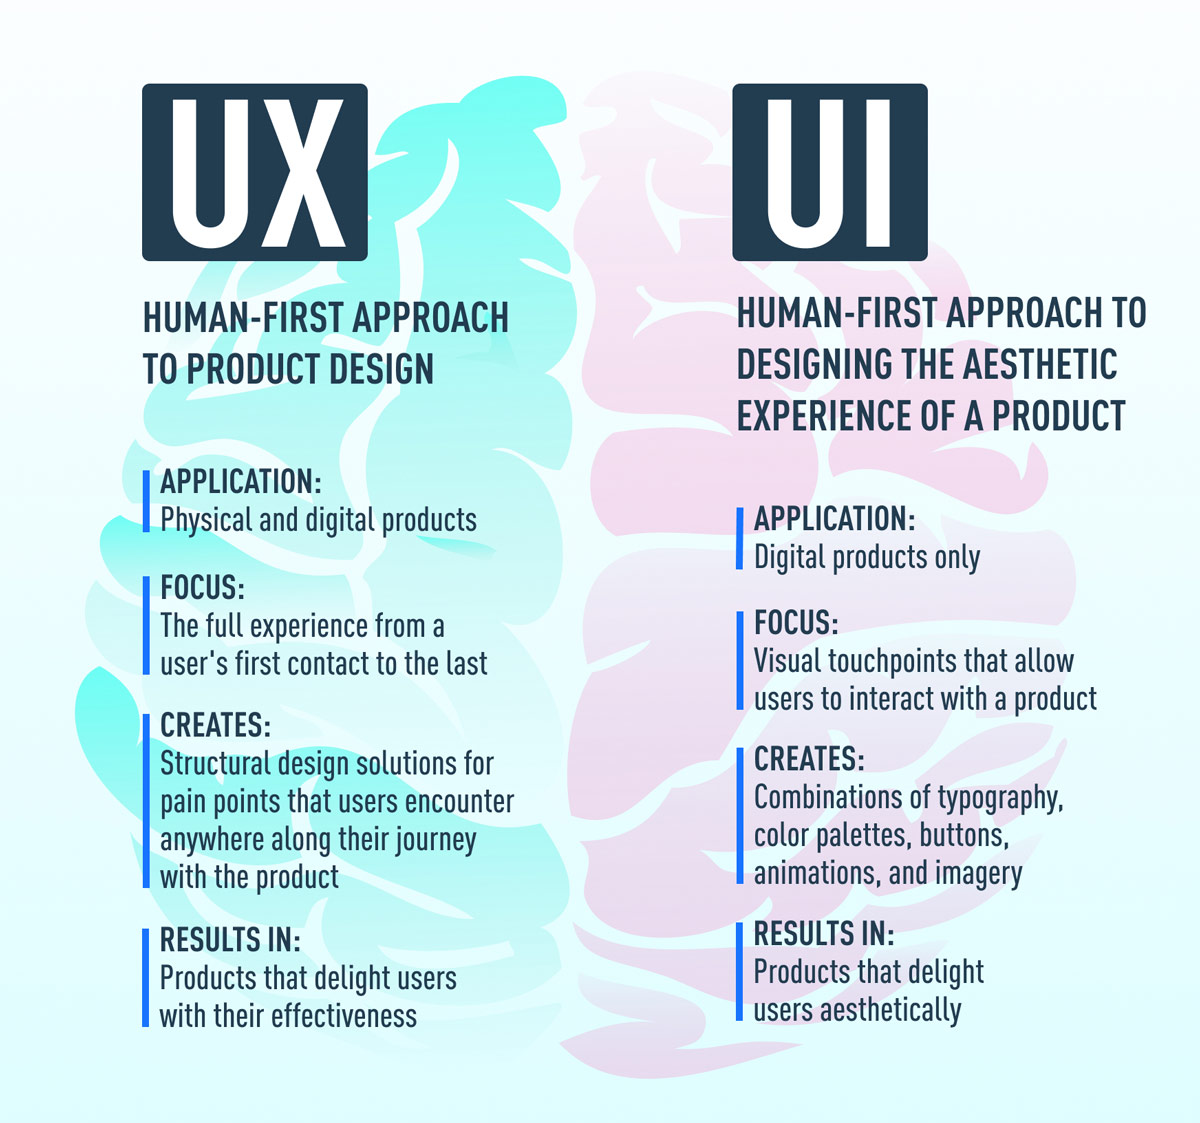
\includegraphics[width=0.7\textwidth]{images/difference-between-ux-and-ui.jpg}
    \caption[Confronto tra la progettazione di interfacce e di esperienze utente]{Confronto tra la progettazione di interfacce (\textit{UI}) e di esperienze utente (\textit{UX})\footnotemark}
\end{figure}
\footnotetext{Fonte: \href{https://careerfoundry.com/en/blog/ux-design/the-difference-between-ux-and-ui-design-a-laymans-guide/}{https://careerfoundry.com}}
Abbiamo svolto degli incontri aggiuntivi in forma telematica per chiarire alcuni aspetti del progetto, in particolare la comprensione di alcuni requisiti utente e la definizione di determinati aspetti 
di interfaccia grafica ed esperienza utente (ovvero come l'utente può interagire con l'interfaccia grafica, la relazione che intercorre tra essi). \\
Per tutta la durata delle attività di \textit{stage}, sono stato affiancato in caso di necessità da praticamente tutto il \textit{team \textbf{Trizeta}}, soprattutto per quanto concerne la progettazione dell'interfaccia grafica.

\section{Strumenti utilizzati}
% In questa sezione descriverò gli strumenti utilizzati nel corso del progetto, suddividendoli in base alle attività in cui essi sono stati impiegati.

\subsection{Strumenti di sviluppo}
    \subsubsection*{Angular}
        \begin{itemize}
            \item [\textit{Versione}:] 16.2.9
            \item [\textit{Descrizione}:] è un \textit{framework open-source} per lo sviluppo di applicazioni \textit{web} a singola pagina (è un tipo di applicazione \textit{web} che opera all'interno di una singola pagina \textit{web}, senza la necessità di ricaricarla durante l'interazione dell'utente). \\ 
                    Sviluppato da \textit{Google}, \textit{Angular} fornisce una struttura per la costruzione di applicazioni \textit{web} dinamiche e interattive, consentendo agli sviluppatori di utilizzare il linguaggio \textit{TypeScript} o \textit{JavaScript} per la creazione di componenti riutilizzabili.
        \end{itemize}
    \subsubsection*{Angular Material}
    \begin{itemize}
        \item [\textit{Versione}:] 16.2.8
        \item [\textit{Descrizione}:] è una libreria di componenti grafiche e direttive, sviluppata da \textit{Google} e progettata per essere utilizzata con il \textit{framework Angular}. \\
                     Questa libreria fornisce una serie di componenti predefiniti e stilizzati che semplificano la creazione di interfacce utente coerenti e moderne all'interno delle applicazioni \textit{Angular}.
    \end{itemize}

    \subsubsection*{Figma}
    \begin{itemize}
        \item [\textit{Versione}:] 9.0
        \item [\textit{Descrizione}:] è un'applicazione di progettazione e prototipazione basata su cloud (\textit{software} il cui funzionamento e archiviazione dei dati avvengono prevalentemente attraverso risorse di calcolo e archiviazione disponibili su \textit{Internet}, anziché su risorse locali o \textit{server} fisici) 
                    che consente di collaborare in tempo reale su progetti di interfaccia utente (\textit{UI}) ed esperienza utente (\textit{UX}).
    \end{itemize}

    \subsubsection*{Karma}
    \begin{itemize}
        \item [\textit{Versione}:] 6.4.0
        \item [\textit{Descrizione}:] è uno strumento ampiamente utilizzato per l'esecuzione di \textit{test} di unità per applicazioni \textit{Angular}. \\
                    \textit{Karma} genera un \textit{server web} che esegue il codice di \textit{test Javascript} (e \textit{TypeScript}, che ne è sovralinguaggio) per ogni \textit{browser} connesso.
    \end{itemize}

    \subsubsection*{Node.js}
    \begin{itemize}
        \item [\textit{Versione}:] 18.17.1
        \item [\textit{Descrizione}:] è un ambiente di \textit{runtime open source} basato sul motore \textit{JavaScript} V8 di \textit{Google Chrome}. \\
                    Consente di eseguire codice \textit{JavaScript} lato \textit{server}, consentendo agli sviluppatori di utilizzare \textit{JavaScript} per lo sviluppo di applicazioni \textit{back-end}.
    \end{itemize}

    \subsubsection*{Ng-openapi-gen}
    \begin{itemize}
        \item [\textit{Versione}:] 0.50.2
        \item [\textit{Descrizione}:] è un modulo \textit{npm} (il gestore di pacchetti per \textit{Node.js}) che genera servizi, 
                    modelli e funzioni \textit{Angular} a partire da una specifica \textit{OpenAPI 3} (è uno \textit{standard} che aiuta a descrivere e documentare le Interfacce di Programmazione delle Applicazioni, \glslink{apig}{\textit{API}}).
    \end{itemize}

    \subsubsection*{Ngx-translate}
    \begin{itemize}
        \item [\textit{Versione}:] 15.0.0
        \item [\textit{Descrizione}:] liberia che consente l'internazionalizzazione in \textit{Angular} (ovvero facilita l'astrazione del contenuto statico di un'applicazione \textit{web} rispetto alla lingua di fruizione).
    \end{itemize}

    \subsubsection*{StarUML}
    \begin{itemize}
        \item [\textit{Versione}:] 6.0.1
        \item [\textit{Descrizione}:] è uno strumento di modellazione \textit{UML}\footnote{\glslink{umlg}{\textit{Unified Modeling Language}}} (\textit{Unified Modeling Language}) che offre un ambiente grafico per progettare e visualizzare diagrammi \glslink{umlg}{\textit{UML}}. \\
                \glslink{umlg}{\textit{UML}} è uno \textit{standard} per la modellazione visuale di sistemi \textit{software}, ed è utilizzato per rappresentare graficamente diversi aspetti di un sistema, come classi, casi d'uso, sequenze, attività, e altro ancora.
    \end{itemize}

    \subsubsection*{TypeScript}
    \begin{itemize}
        \item [\textit{Versione}:] 5.1.6
        \item [\textit{Descrizione}:] è un linguaggio di programmazione \textit{open-source} sviluppato da \textit{Microsoft}. \\
                È una versione "\textit{superset}" di \textit{JavaScript}, il che significa che aggiunge nuove funzionalità e tipizzazione statica al linguaggio JavaScript.
    \end{itemize}

    \subsubsection*{Visual Studio Code}
    \begin{itemize}
        \item [\textit{Versione}:] 1.84.1
        \item [\textit{Descrizione}:] è un \textit{editor} di codice sorgente gratuito e \textit{open-source} sviluppato da \textit{Microsoft}. \\
                È progettato per essere leggero, flessibile e altamente personalizzabile, rendendolo uno strumento popolare tra gli sviluppatori per la scrittura di codice in diversi linguaggi di programmazione.
    \end{itemize}


\subsection{Strumenti di versionamento}
    \subsubsection*{Git}
    \begin{itemize}
        \item [\textit{Versione}:] 2.43.0
        \item [\textit{Descrizione}:] è un sistema di controllo delle versioni distribuito (\textit{DVCS}), utilizzato per tracciare le modifiche apportate al codice sorgente durante lo sviluppo del \textit{software}.
    \end{itemize}

    \subsubsection*{GitHub}
    \begin{itemize}
        \item [\textit{Versione}:] 3.11.0
        \item [\textit{Descrizione}:] è una piattaforma di \textit{hosting} per il controllo delle versioni e la collaborazione. \\
                    Offre servizi basati su \textit{Git} e facilita la gestione e la condivisione dei progetti \textit{software}.
    \end{itemize}

\subsection{Strumenti di documentazione}

\subsubsection*{Compodoc}
\begin{itemize}
    \item [\textit{Versione}:] 1.1.22
    \item [\textit{Descrizione}:] strumento \textit{open-source} per la generazione di documentazione per \textit{web app Angular} a partire da commenti scritti nel codice sorgente.
\end{itemize}

\subsubsection*{LibreOffice}
\begin{itemize}
    \item [\textit{Versione}:] 7.6.2
    \item [\textit{Descrizione}:] è una \textit{suite} di \textit{software} per l'ufficio libera e \textit{open-source} che offre un insieme di applicazioni per la produttività personale e professionale. \\
                È sviluppato dalla comunità di sviluppatori di \textit{The Document Foundation} ed è una delle alternative più popolari e complete a \textit{suite} di produttività come \textit{Microsoft Office}.
\end{itemize}

\section{Analisi dei requisiti utente}

In questa sezione descriverò lo scopo dell'analisi dei requisiti in un progetto, le problematiche riscontrate e mostrerò i principali casi d'uso ed i principali requisiti elaborati.

\section{Progettazione}

In questa sezione descriverò lo scopo della progettazione in un progetto, le problematiche riscontrate e mostrerò le classi (e le loro dipendenze, quando utile e possibile, tramite il linguaggio UML) relative ai principali requisiti analizzati nella sezione precedente in modo da dare riscontro effettivo del passaggio da "requisito" a "scelta progettuale".
In questa sezione includerò anche la progettazione dell'interfaccia grafica relativa alle classi sopra indicate.

% fare commenti su internazionalizzazione e localizzazione
\section{Codifica}

In questa sezione descriverò lo scopo della codifica in un progetto ed indicherò le problematiche riscontrate.

\section{Verifica}

In questa sezione descriverò le modalità con le quali si è accertato che l’esecuzione delle attività (per un determinato periodo di tempo) non abbia introdotto errori.

\section{Validazione}

In questa sezione descriverò le modalità con le quali si è accertato che il prodotto finito fosse conforme alle aspettative.

\section{Statistiche qualitative e quantitative finali}

In questa sezione descriverò i prodotti di progetto dal punto di vista della qualità (qui vi sarà particolare enfasi sul prodotto software) e della quantità.